\chapter{Specification of needs}
\section*{Introduction}
In this chapter, we will identify the actors, then we will specify the functional and non-functional needs that the proposed solution must meet. Finally, we present the use case diagrams explaining our application's main functionalities.
\section{Identification of actors}
An actor represents an external entity that interacts directly with the
system. It can be either a human person or a system. We distinguish
two types of actors, the main actor, and a secondary actor. Indeed,
a principal actor obtains an observable result of the system while a
secondary actor is asked for additional information.\\
\subsection*{Main actors}
\textbf{Community Manager \& Salesforce Administrator}\\
Both the community manager and the Salesforce Administrator are the main users of our application and should be able to :
\begin{itemize}
\item[•] Choose the community that he has the right to access and manage.
\item[•] Consult users of a specific community inside a well-organized table with pagination options.
\item[•] Filter said users by name, user-name, Salesforce account name, status (active or not active), and Salesforce profile.
\item[•] Consult and update the details of each user.
\item[•] Activate users within a specific community.
\item[•] Deactivate users within a specific community.
\item[•] Send a "Welcome to community" email to a specific active user.
\item[•] Send a "Reset password" email to a specific active user.
\item[•] Consult a bar chart showing each user's logins within the selected community.
\item[•] Filter chart results by the period between two specific dates.
\item[•] Consult details about each user displayed in the chart.
\item[•] Update the Salesforce user license for each user displayed in the chart.
\item[•] Consult users failed login attempts to a specific community inside a well-organized table with pagination options.
\item[•] Filter said login attempts by name, user-name, status( Invalid password, No community access, etc... ) and event date and time.
\item[•] Consult detailed information about each login attempt.
\item[•] Send a security warning email to the account owner about the login attempt event.
\item[•] Access a Chatbot that provides information about the selected community or the Salesforce organization.
\item[•] Access a synthetic dashboard displaying community KPIs (Key Performance Indicators).

\end{itemize}
In case when the community manager or the Salesforce Administrator has a Salesforce role he will be also able to :
\begin{itemize}
\item[•] Add one or multiple users to a specific community at once.
\end{itemize}

\subsection*{Secondary actors}
\textbf{Salesforce System}\\
This actor is the system, previously developed and deployed in a cloud server by the Salesforce organization, interactable through our application, and it's responsible for :
\begin{itemize}
\item[•] Sending an automatic "Welcome to community" email upon adding a new member to the community by our application user.  
\item[•] Sending an automatic "Welcome to community" email upon activating a previously deactivated user by our application user.
\item[•] Generating reset password URL upon sending a "Reset password" email to a community member by our application user.
\item[•] Tracking users' successful and failed login attempts and saving them to the organization database.

\end{itemize}
\section{Functional Needs}
Functional needs are expressed by the user of the application
which makes it possible to identify the functionalities of this application.\\
In our
case, the functional needs are:
\begin{itemize}
\item Choice of the community:\\
Select the community to which we will manage the users.

\item Manage users:\\
The system must allow users to be managed with the functionalities of activation,
deactivation, modification, and consultation of the list of users via a data table.
Creation of different filters that allow us to facilitate the navigation of the list of users.

\item Manage connection history:\\
Create a chart that shows the number of user connections per day, week, year, or
according to a well-determined date. This allows the administrator to modify the user’s license.


\item Offer a synthetic dashboard:\\
Allowing the system administrator / the community manager to visualize the KPIs (Key Performance Indicators) of his organization/community.

\item Manage failed login attempts:\\
Allowing the system administrator / the community manager to consult details about failed login events as well as send security warning emails to concerned users.

\item Access a smart Chatbot:\\
Allowing the system administrator / the community manager to request pieces of information from a smart digital assistant.


\end{itemize}
\section{Non-functional Needs}
Non-functional requirements represent the characteristics of the system.
They relate to the constraints to be taken into consideration to set up
an adequate solution.\\
For our application, the non-functional requirements are:
\begin{itemize}
\item Security:\\
Access to information is only possible after verification of privileges and access rights,
for example Authentication, Redirections.

\item Ergonomics and user-friendliness:\\
The application will provide a user-friendly and easy-to-use interface that does not
require any prerequisites, so it can be used by all types of users (even non-computer specialists).

\item Extensibility and maintainability:\\
The architecture of the application will allow the evolution and maintenance (addition
or deletion or update) at the level of its various modules in a flexible manner.

\item Performance:\\
The application must be efficient, i.e. the system must react within a period that does
not exceed 5 seconds, whatever the action of the application.

\item Availability:\\
The application will be available on 24/24 and 7/7 except during maintenance.

\end{itemize}
\section{Use case diagrams}
In this section, we will highlight the system's functionalities to be
from the functional needs mentioned above based on the UML(Unified Modeling Language) diagrams which group together all the system's use cases.
\subsection{Global use case diagram}
The figure \ref{global_uc} illustrates the global use case diagram of our application
\begin{figure}[H]%
    \center   
    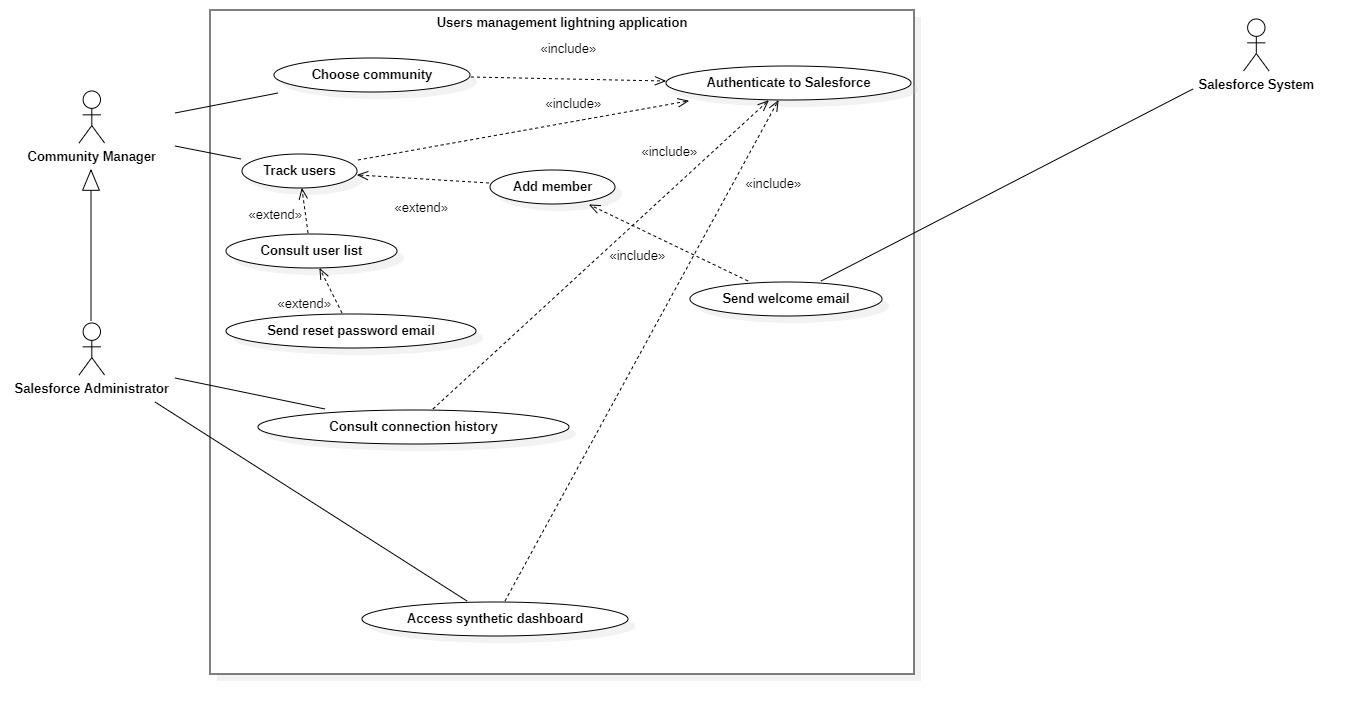
\includegraphics[scale=0.45]{Global UC.jpg}
    \caption{Global use case diagram}
    \label{global_uc}
\end{figure}
Our application will provide both the community manager and the system administrator ,as long as they are authenticated to Salesforce, the ability to:
\begin{itemize}
\item Search for and select the community that they want to manage.
\item Track community members by either consult the full user list or add new members, as long as they own a Salesforce role, where the Salesforce system will send an automatic welcome email to the new community member.
\item Access synthetic dashboard illustrating the KPI (Key Performance Indicators) of the community.
\item Access a smart Chatbot that will provide useful Salesforce information to the user.
\item Consult and manage failed login attempts committed by community members and previously recorded and stored by the Salesforce system.
\item Consult and filter members' connection history previously recorded and stored by the Salesforce system, as well as update their Salesforce license to match their level of activity.
\end{itemize}
\subsection{Use case refinement}
In this section, we will detail the main use cases.
\subsubsection{Consult user list use case refinement}
In our application, the community manager and the system administrator can access a data table containing the full list of users within their respective communities.\\
The figure \ref{userlist_uc} shows the Consult user list use case diagram.
\begin{figure}[H]%
    \center   
    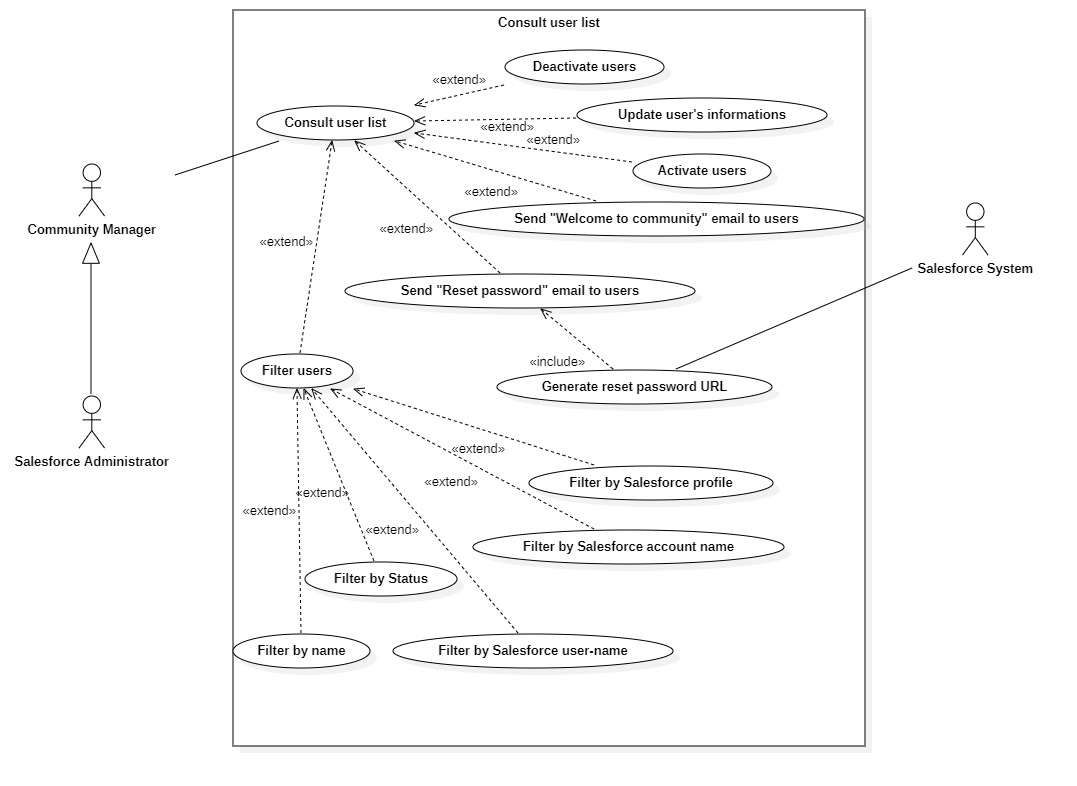
\includegraphics[scale=0.5]{Consult users list UC.jpg}
    \caption{Consult user list use case diagram}
    \label{userlist_uc}
\end{figure}
The table \ref{userlist_table} details the tasks to be performed by the user to manage the user list.

\begin{table}[H]
\footnotesize% or \small or \scriptsize
\begin{tabular}{|ll|}
\hline
\multicolumn{2}{|c|}{\textbf{Summary}}                                                                                                                                                                                                                                                                                                                                                                                                                                                                                                                                                                                                                                                                                                                                                         \\ \hline
\multicolumn{1}{|l|}{Title}                      & Consult user list                                                                                                                                                                                                                                                                                                                                                                                                                                                                                                                                                                                                                                                                                                                           \\ \hline
\multicolumn{1}{|l|}{Objectif}                   & \begin{tabular}[c]{@{}l@{}}Allowing the community manager or the system administrator\\ to manage his community members\end{tabular}                                                                                                                                                                                                                                                                                                                                                                                                                                                                                                                                                                                                        \\ \hline
\multicolumn{1}{|l|}{Actors}                     & Community manager, System administrator                                                                                                                                                                                                                                                                                                                                                                                                                                                                                                                                                                                                                                                                                                     \\ \hline
\multicolumn{2}{|c|}{\textbf{Description of sequences}}                                                                                                                                                                                                                                                                                                                                                                                                                                                                                                                                                                                                                                                                                                                                        \\ \hline
\multicolumn{1}{|l|}{Pre-condition}              & \begin{tabular}[c]{@{}l@{}}- User should be authenticated to Salesforce\\ - User should be the owner of at least one community\end{tabular}                                                                                                                                                                                                                                                                                                                                                                                                                                                                                                                                                                                                 \\ \hline
\multicolumn{1}{|l|}{Post-condition}             & - Community members are well organized                                                                                                                                                                                                                                                                                                                                                                                                                                                                                                                                                                                                                                                                                                      \\ \hline
\multicolumn{1}{|l|}{Normal scenario}            & \begin{tabular}[c]{@{}l@{}}1. User accesses the user list interface\\ 2. User selects one or many community members\\ 3. User clicks the "activate/deactivate" button for selected members\\ 4. The system prompts the success of the operation\\ 5. The user clicks the "Send welcome email" button\\ for the selected members\\ 6. The system prompts the success of the operation\\ 7. The user clicks the "Send reset password" button\\ for the selected members\\ 8. The system prompts the success of the operation\\ 9. The user clicks the "show details" button for one member\\ 10. The member information interface pops up \\ 11. User updates the selected member information and complies\\ 12. System prompts the success of the operation\end{tabular} \\ \hline
\multicolumn{1}{|l|}{Alternative scenario}       & \begin{tabular}[c]{@{}l@{}}1. License limit exceeded when activating members: The system\\ sends an error message\\ 2. Sending a welcome email to a deactivated member: The system\\ sends an error message\\ 3. Changing member username to an existing one: The system\\ sends an error message\end{tabular}                                                                                                                                                                                                                                                                                                                                                                                                                              \\ \hline
\multicolumn{1}{|l|}{Non-functional constraints} & \begin{tabular}[c]{@{}l@{}}1. The interface must be ergonomic\\ 2. Error messages should be understandable and clear\end{tabular}                                                                                                                                                                                                                                                                                                                                                                                                                                                                                                                                                                                                           \\ \hline
\end{tabular}
\captionsetup{skip=5pt} % Adjust the skip value as per your needs
\caption{Consult user list use case}
\label{userlist_table}

\end{table}
\pagebreak
\subsubsection{Add members use case refinement}
In our application, the community manager and system administrator can add one or multiple members to their respective communities at once.\\

The table \ref{addmembers_table} details the tasks to be performed by the user to add members to his community.

\begin{table}[H]

\begin{tabular}{|ll|}
\hline
\multicolumn{2}{|c|}{\textbf{Summary}}                                                                                                                                                                                                                                                                                                                                                                                                                                                                                                                                                                                                                                                                                      \\ \hline
\multicolumn{1}{|l|}{Title}                      & Add members                                                                                                                                                                                                                                                                                                                                                                                                                                                                                                                                                                                                                                                              \\ \hline
\multicolumn{1}{|l|}{Objectif}                   & \begin{tabular}[c]{@{}l@{}}Allowing the community manager or the system administrator to \\ add one or multiple members at once to his community\end{tabular}                                                                                                                                                                                                                                                                                                                                                                                                                                                                                                            \\ \hline
\multicolumn{1}{|l|}{Actors}                     & Community manager, System administrator                                                                                                                                                                                                                                                                                                                                                                                                                                                                                                                                                                                                                                  \\ \hline
\multicolumn{2}{|c|}{\textbf{Description of sequences}}                                                                                                                                                                                                                                                                                                                                                                                                                                                                                                                                                                                                                                                                     \\ \hline
\multicolumn{1}{|l|}{Pre-condition}              & \begin{tabular}[c]{@{}l@{}}- User should be authenticated to Salesforce\\ - User should be the owner of at least one community\\ - User should have a Salesforce role\end{tabular}                                                                                                                                                                                                                                                                                                                                                                                                                                                                                       \\ \hline
\multicolumn{1}{|l|}{Post-condition}             & - New member(s) are added to the owner's community                                                                                                                                                                                                                                                                                                                                                                                                                                                                                                                                                                                                                       \\ \hline
\multicolumn{1}{|l|}{Normal scenario}            & \begin{tabular}[c]{@{}l@{}}1. User accesses the add members interface\\ 2. The user fills the displayed form with information about the new member\\ 3. The user clicks the " add another member" button\\ 4. A new empty form, identical to the previous one, is displayed\\ 5. The user fills the new form with information about the next new member\\ 6. The user clicks the "clone member" button\\ 7. A new form containing the same values as the previous form is displayed\\ 8. The user clicks the "delete form" button\\ 9. The selected form is deleted from the screen\\ 10. The user clicks the "submit" button \\ 11. System prompts the success of the operations\end{tabular} \\ \hline
\multicolumn{1}{|l|}{Alternative scenario}       & \begin{tabular}[c]{@{}l@{}}1. Empty fields: The system sends an error message:\\ You must complete all the required fields\\ 2. The email entered is not valid: The system sends an error message\\ describing the validation conditions for this field\\ 3. Duplicate Salesforce user-name: The system sends an error message\end{tabular}                                                                                                                                                                                                                                                                                                                              \\ \hline
\multicolumn{1}{|l|}{Non-functional constraints} & \begin{tabular}[c]{@{}l@{}}1. The interface must be ergonomic\\ 2. Error messages should be understandable and clear\end{tabular}                                                                                                                                                                                                                                                                                                                                                                                                                                                                                                                                        \\ \hline
\end{tabular}
\captionsetup{skip=5pt} % Adjust the skip value as per your needs
\caption{Add members use case}
\label{addmembers_table}

\end{table}
\subsubsection{Consult synthetic dashboard use case refinement}
In our application, the community manager and the system administrator can access a dashboard containing features that helps them to manage their respective communities.\\
The figure \ref{dashboard_uc} shows the "Consult synthetic dashboard" use case diagram.
\begin{figure}[H]%
    \center   
    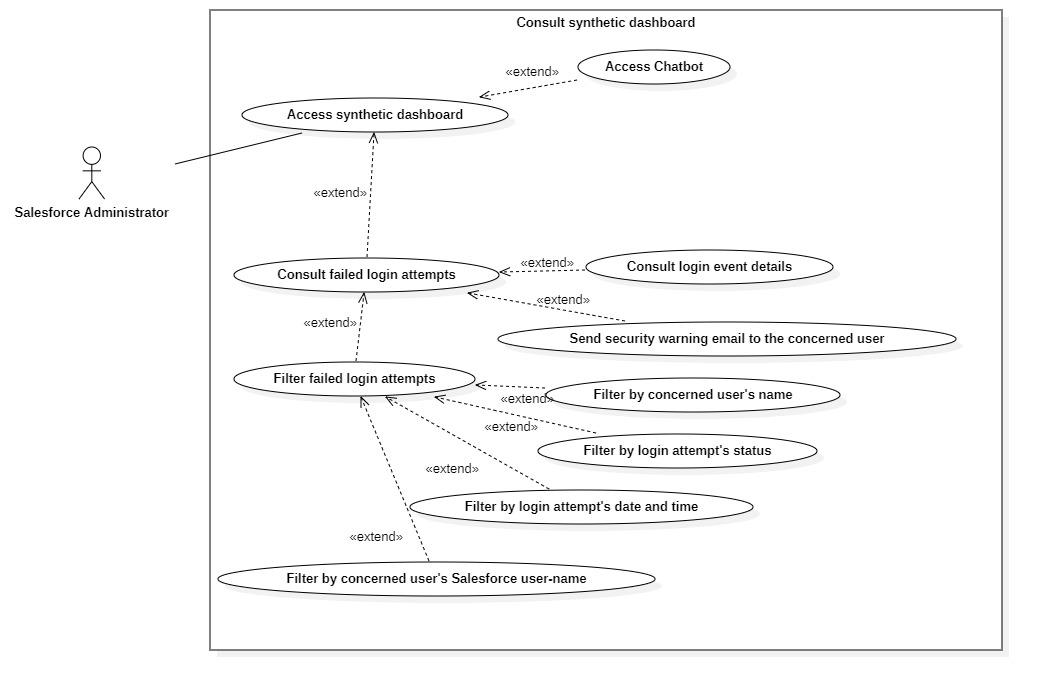
\includegraphics[scale=0.5]{Consult synthetic dashboard UC.jpg}
    \caption{Consult synthetic dashboard use case diagram}
    \label{dashboard_uc}
\end{figure}

The table \ref{dashboard_table} details the tasks to be performed by the customer to consult the synthetic dashboard
in our application.
\begin{table}[H]

\begin{tabular}{|ll|}
\hline
\multicolumn{2}{|c|}{\textbf{Summary}}                                                                                                                                                                                       \\ \hline
\multicolumn{1}{|l|}{Title}                      & Consult synthetic dashboard                                                                                                                                               \\ \hline
\multicolumn{1}{|l|}{Objectif}                   & \begin{tabular}[c]{@{}l@{}}Allowing the system administrator\\ to access extra features that helps him to manage his communities\end{tabular} \\ \hline
\multicolumn{1}{|l|}{Actors}                     & System administrator, Community Manager                                                                                                                                   \\ \hline
\multicolumn{2}{|c|}{\textbf{Description of sequences}}                                                                                                                                                                      \\ \hline
\multicolumn{1}{|l|}{Pre-condition}              & \begin{tabular}[c]{@{}l@{}}- User should be authenticated to Salesforce\\ - User should be the owner of at least one community\end{tabular}                               \\ \hline
\multicolumn{1}{|l|}{Post-condition}             & \begin{tabular}[c]{@{}l@{}}- System administrator is well informed\\ about his respective community's KPIs.\end{tabular}                                \\ \hline
\multicolumn{1}{|l|}{Normal scenario}            & \begin{tabular}[c]{@{}l@{}}1. User accesses the dashboard interface\\ 2. Multiple KPI charts pop up \\ 3. Users may click a bar from the developers' Error Metrics Chart\\ to access error logs specific to the selected developer \end{tabular}       \\ \hline
\multicolumn{1}{|l|}{Alternative scenario}       &                                                                                                                                                                           \\ \hline
\multicolumn{1}{|l|}{Non-functional constraints} & 1. The interface must be ergonomic                                                                                                                                        \\ \hline
\end{tabular}
\caption{Consult synthetic dashboard use case}
\label{dashboard_table}
\end{table}
\subsubsection{Consult the failed login attempts use case refinement}
In our application, the community manager and the system administrator can manage failed login attempts committed by their community's members as well as send security warning emails containing details about the event to concerned members.\\
The figure \ref{loginattempts_uc} shows the "consult failed login attempts" use case diagrams.
\begin{figure}[H]%
    \center   
    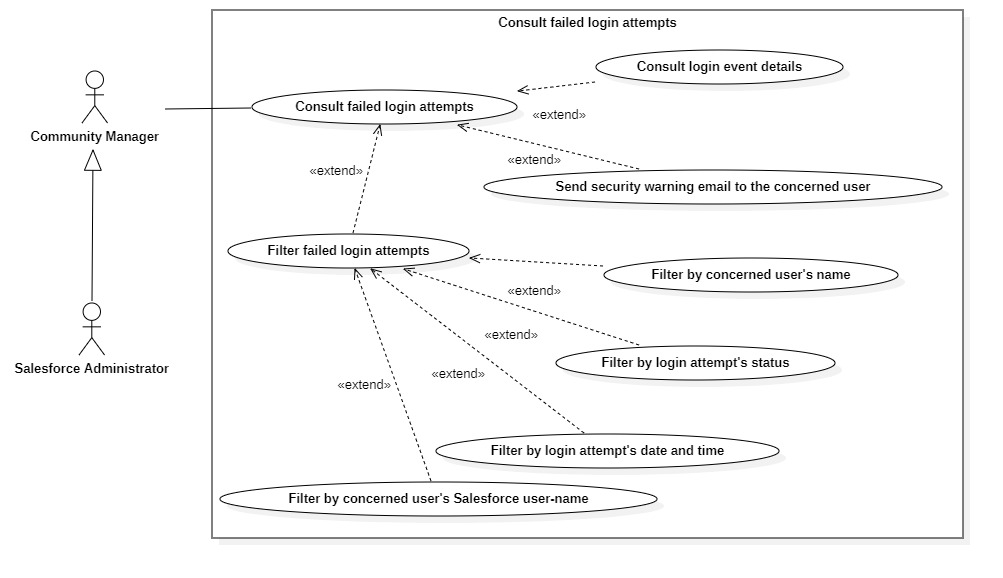
\includegraphics[scale=0.5]{Consult failed login attempts.jpg}
    \caption{Consult failed login attempts use case diagram}
    \label{loginattempts_uc}
\end{figure}

The table \ref{loginattempts_table} details the tasks to be performed by the customer to consult the failed login attempts
in our application.
\begin{table}[H]
\begin{tabular}{|ll|}
\hline
\multicolumn{2}{|c|}{\textbf{Summary}}                                                                                                                                                                                                                                                                                                                                                                                                                                                                                                                           \\ \hline
\multicolumn{1}{|l|}{Title}                      & Consult failed login attempts                                                                                                                                                                                                                                                                                                                                                                                                                                                                                 \\ \hline
\multicolumn{1}{|l|}{Objectif}                   & \begin{tabular}[c]{@{}l@{}}Allowing  the system administrator\\ to access failed login attempts and inform concerned users about them\end{tabular}                                                                                                                                                                                                                                                                                                                                                            \\ \hline
\multicolumn{1}{|l|}{Actors}                     & System administrator, Community manager                                                                                                                                                                                                                                                                                                                                                                                                                                                                                          \\ \hline
\multicolumn{2}{|c|}{\textbf{Description of sequences}}                                                                                                                                                                                                                                                                                                                                                                                                                                                                                                          \\ \hline
\multicolumn{1}{|l|}{Pre-condition}              & \begin{tabular}[c]{@{}l@{}}- User should be authenticated to Salesforce\\ - User should be the owner of at least one community\end{tabular}                                                                                                                                                                                                                                                                                                                                                                   \\ \hline
\multicolumn{1}{|l|}{Post-condition}             & - Users are well-informed about their account security status.                                                                                                                                                                                                                                                                                                                                                                                                                                                \\ \hline
\multicolumn{1}{|l|}{Normal scenario}            & \begin{tabular}[c]{@{}l@{}}1. User accesses the failed login attempts interface\\ 2. The user clicks the "show details" button for a specific login event\\ 3. The "show details" interface for the selected login event pops up\\ 4. The user clicks the "send security warning email" button for\\ the specific login event\\ 5. The system prompts the success of the operation\\ 6. The concerned user receives the warning email, containing details\\ about the failed login attempt, in his email\end{tabular} \\ \hline
\multicolumn{1}{|l|}{Alternative scenario}       & \begin{tabular}[c]{@{}l@{}}1. Server error when sending the warning email: The system\\ sends an error message received from the server\end{tabular}                                                                                                                                                                                                                                                                                                                                                          \\ \hline
\multicolumn{1}{|l|}{Non-functional constraints} & \begin{tabular}[c]{@{}l@{}}1. The interface must be ergonomic\\ 2. Error messages should be understandable and clear\end{tabular}                                                                                                                                                                                                                                                                                                                                                                             \\ \hline
\end{tabular}
\caption{Consult failed login attempts use case}
\label{loginattempts_table}
\end{table}



\subsubsection{Access Chatbot use case refinement}
In our application, the community manager and the system administrator can access a smart Chatbot interface to benefit from a Salesforce digital assistant that will provide information about Salesforce and its features as well as provide information about the current community.\\ 
The figure \ref{chatbot_uc} illustrates the use case diagram "Access Chatbot"

\begin{figure}[H]%
    \center   
    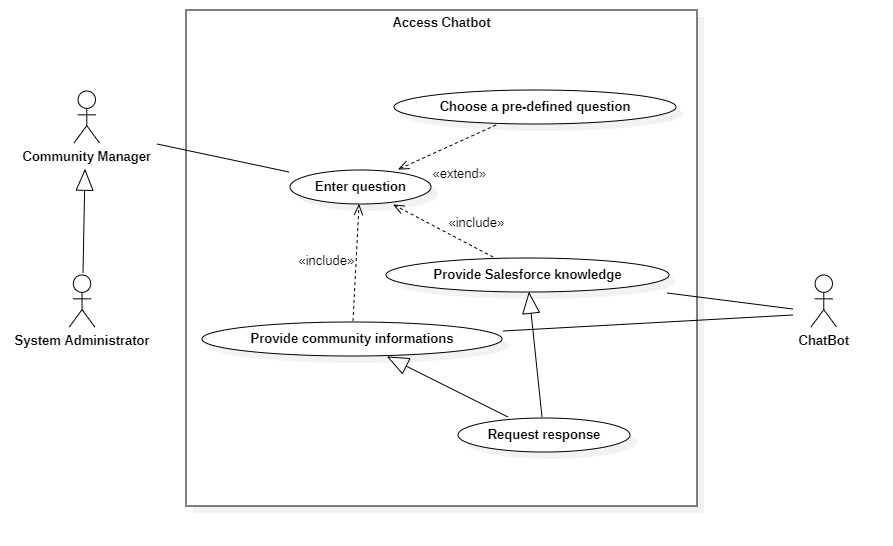
\includegraphics[scale=0.5]{Access Chatbot.jpg}
    \caption{Access Chatbot use case diagram}
    \label{chatbot_uc}
\end{figure}

The table \ref{chatbot_table} details the tasks to be performed by the customer to Access the Chatbot within our app.
\begin{table}[H]
\begin{tabular}{|ll|}
\hline
\multicolumn{2}{|c|}{\textbf{Summary}}                                                                                                                                                                                                                                                                                                                              \\ \hline
\multicolumn{1}{|l|}{Title}                      & Access Chatbot                                                                                                                                                                                                                                                                                                   \\ \hline
\multicolumn{1}{|l|}{Objectif}                   & \begin{tabular}[c]{@{}l@{}}Trigger a Chatbot that responds to user requests \\ while providing informations about the current community\end{tabular}                                                                                                                                                             \\ \hline
\multicolumn{1}{|l|}{Actors}                     & System administrator, Community manager, Chatbot                                                                                                                                                                                                                                                                                    \\ \hline
\multicolumn{2}{|c|}{\textbf{Description of sequences}}                                                                                                                                                                                                                                                                                                             \\ \hline
\multicolumn{1}{|l|}{Pre-condition}              & \begin{tabular}[c]{@{}l@{}}- User should be authenticated to Salesforce\\ - User should be the owner of at least one community\end{tabular}                                                                                                                                                                      \\ \hline
\multicolumn{1}{|l|}{Post-condition}             & \begin{tabular}[c]{@{}l@{}} - User question is answered\\ and the response is displayed on the screen. \end{tabular}                                                                                                                                                                                                                                             \\ \hline
\multicolumn{1}{|l|}{Normal scenario}            & \begin{tabular}[c]{@{}l@{}}1. User accesses the Chatbot interface\\ 2. User types a question or selects a predefined question.\\ 3. The chatbot is launched upon receipt of a request\\ 4. The chatbot analyzes the request\\5. The chatbot prepares the response\\ 6. The chatbot sends the response\end{tabular} \\ \hline
\multicolumn{1}{|l|}{Alternative scenario}       &\begin{tabular}[c]{@{}l@{}} 1. An error message is displayed if the question\\ is not recognized by the system.\end{tabular}                                                                                                                                                                                                                                 \\ \hline
\multicolumn{1}{|l|}{Non-functional constraints} & \begin{tabular}[c]{@{}l@{}}1. The interface must be ergonomic\\ 2. Error messages should be understandable and clear\\ 3. The ChatBot must always be available.\end{tabular}                                                                                                                                     \\ \hline
\end{tabular}

\caption{Access Chatbot use case}
    \label{chatbot_table}

\end{table}

\pagebreak
\section*{Conclusion}
In this chapter, we have described the specification phases of the
needs of our developed application to identify the different actors
as well as the features and services that our application must provide.\\
We have detailed these features with use case diagrams. The next chapter will be devoted to the conception phase.